\documentclass[tikz,border=5mm]{standalone}
\usepackage{fontspec}
\setmainfont{Times New Roman}
\usetikzlibrary{arrows.meta, positioning, calc, fit, backgrounds}

% Explicitly define layers to fix any hidden background box rendering bugs
\pgfdeclarelayer{background}
\pgfsetlayers{background,main}

\begin{document}
\rmfamily
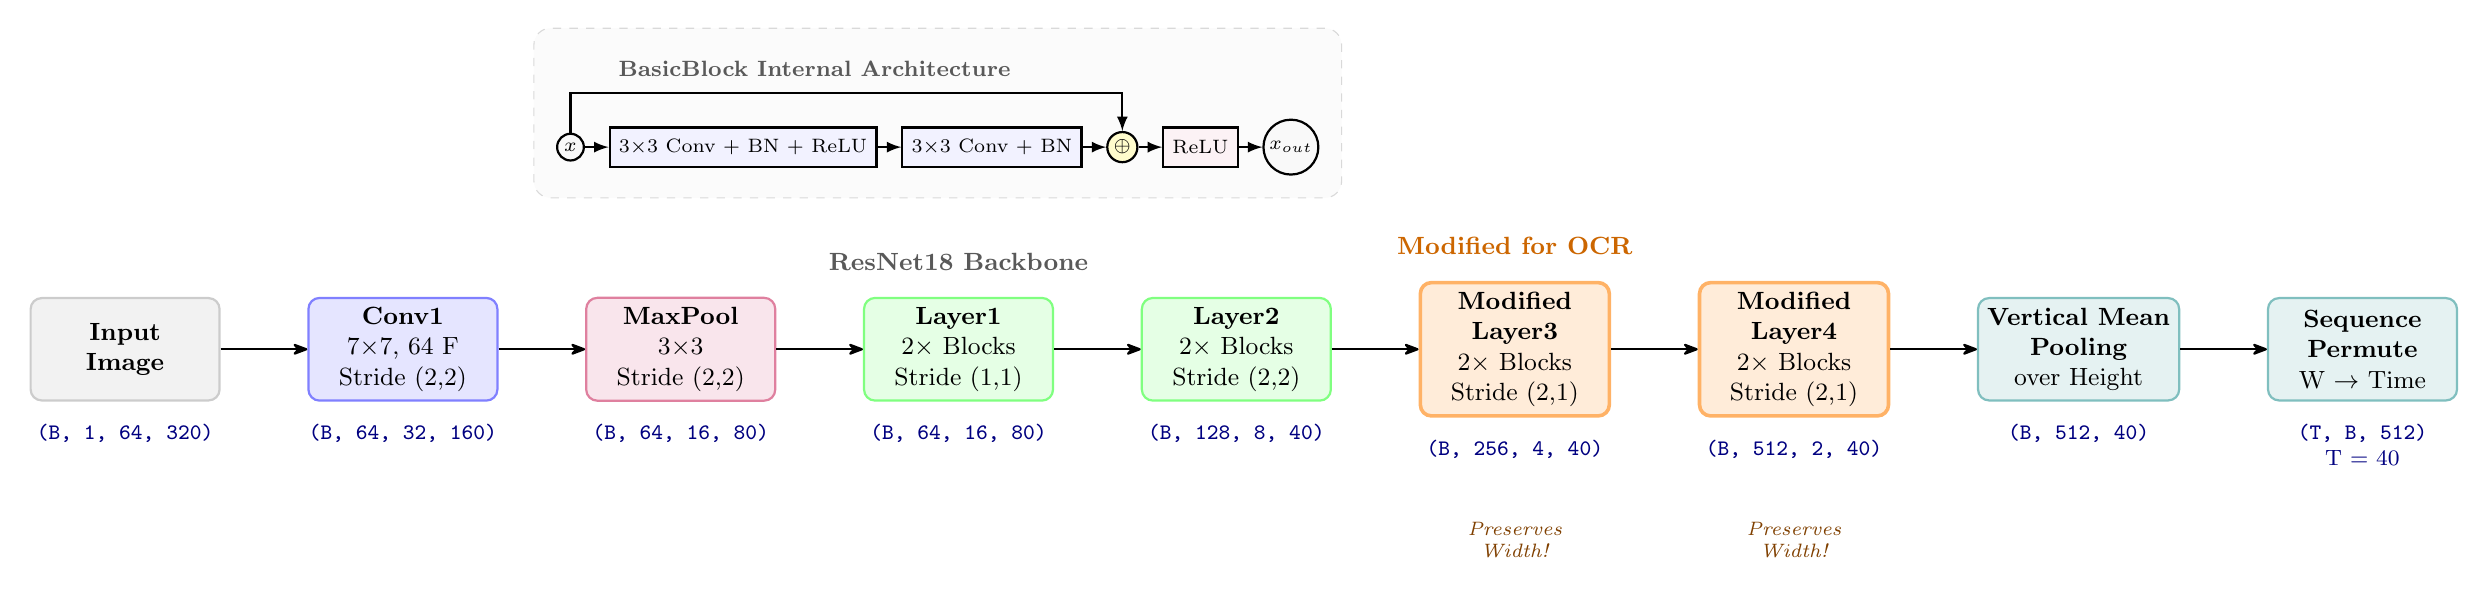
\begin{tikzpicture}[
    thick,
    % Horizontal node distance optimized to give everything breathing room
    node distance=1.0cm and 1.1cm,
    % Core layer box styling
    base/.style={
        draw, 
        minimum width=2.4cm, 
        minimum height=1.3cm, 
        align=center, 
        font=\small\bfseries, 
        rounded corners=4pt,
        line width=0.8pt
    },
    input/.style={base, fill=gray!10, draw=gray!40},
    conv/.style={base, fill=blue!10, draw=blue!50},
    pool/.style={base, fill=purple!10, draw=purple!50},
    normal_res/.style={base, fill=green!10, draw=green!50},
    mod_res/.style={base, fill=orange!15, draw=orange!60, line width=1.3pt},
    post/.style={base, fill=teal!10, draw=teal!50},
    % Typography helpers
    shape_node/.style={font=\footnotesize\ttfamily\color{blue!50!black}, align=center},
    note_node/.style={font=\scriptsize\itshape\color{orange!50!black}, align=center},
    >={Stealth[round]}
]

    % ==========================================
    % 1. MAIN HORIZONTAL PIPELINE
    % ==========================================
    
    % Input Layer
    \node[input] (in) {Input\\Image};
    \node[shape_node, below=0.15cm of in] (s_in) {(B, 1, 64, 320)};
    
    % Stem Stage (FIXED: Cleaned up the broken dollar sign math syntax)
    \node[conv, right=of in] (conv1) {Conv1\\{\normalfont 7$\times$7, 64 F}\\\normalfont Stride (2,2)};
    \node[shape_node, below=0.15cm of conv1] (s_c1) {(B, 64, 32, 160)};
    
    \node[pool, right=of conv1] (maxpool) {MaxPool\\{\normalfont 3$\times$3}\\\normalfont Stride (2,2)};
    \node[shape_node, below=0.15cm of maxpool] (s_mp) {(B, 64, 16, 80)};
    
    % Standard ResNet18 Layers (Updated to 2x Blocks)
    \node[normal_res, right=of maxpool] (lay1) {Layer1\\{\normalfont 2$\times$ Blocks}\\\normalfont Stride (1,1)};
    \node[shape_node, below=0.15cm of lay1] (s_l1) {(B, 64, 16, 80)};
    
    \node[normal_res, right=of lay1] (lay2) {Layer2\\{\normalfont 2$\times$ Blocks}\\\normalfont Stride (2,2)};
    \node[shape_node, below=0.15cm of lay2] (s_l2) {(B, 128, 8, 40)};
    
    % Modified ResNet18 Layers (OCR Specific - Updated to 2x Blocks)
    \node[mod_res, right=of lay2] (lay3) {Modified\\Layer3\\{\normalfont 2$\times$ Blocks}\\\normalfont Stride (2,1)};
    \node[shape_node, below=0.15cm of lay3] (s_l3) {(B, 256, 4, 40)};
    \node[note_node, below=0.55cm of s_l3] (n_l3) {Preserves\\Width!};
    
    \node[mod_res, right=of lay3] (lay4) {Modified\\Layer4\\{\normalfont 2$\times$ Blocks}\\\normalfont Stride (2,1)};
    \node[shape_node, below=0.15cm of lay4] (s_l4) {(B, 512, 2, 40)};
    \node[note_node, below=0.55cm of s_l4] (n_l4) {Preserves\\Width!};
    
    % Sequence Transition Head
    \node[post, right=of lay4] (pool2d) {Vertical Mean\\Pooling\\{\normalfont over Height}};
    \node[shape_node, below=0.15cm of pool2d] (s_p2d) {(B, 512, 40)};
    
    \node[post, right=of pool2d] (reshape) {Sequence\\Permute\\{\normalfont W $\to$ Time}};
    \node[shape_node, below=0.15cm of reshape] (s_resh) {(T, B, 512)\\{\normalfont T = 40}};

    % Main Line Connections
    \draw[->] (in) -- (conv1);
    \draw[->] (conv1) -- (maxpool);
    \draw[->] (maxpool) -- (lay1);
    \draw[->] (lay1) -- (lay2);
    \draw[->] (lay2) -- (lay3);
    \draw[->] (lay3) -- (lay4);
    \draw[->] (lay4) -- (pool2d);
    \draw[->] (pool2d) -- (reshape);

    % Upper Category Architecture Labels
    \node[font=\small\bfseries\color{gray!70!black}, above=0.2cm of lay1] {ResNet18 Backbone};
    \node[font=\small\bfseries\color{orange!80!black}, above=0.2cm of lay3] {Modified for OCR};

    % ==========================================
    % 2. COMPACT RESIDUAL BASICBLOCK INSET
    % ==========================================
    \begin{scope}[shift={($(maxpool.north) + (-1.4, 1.7)$)}]
        % Main title for the block breakdown
        \node[font=\footnotesize\bfseries, text=gray!70!black] (bbtitle) at (3.1, 1.2) {BasicBlock Internal Architecture};
        
        % Block nodes
        \node[circle, draw, fill=gray!5, inner sep=1.5pt, font=\scriptsize] (xi) at (0, 0.2) {$x$};
        \node[draw, fill=blue!5, font=\scriptsize, minimum height=0.5cm, right=0.3cm of xi] (c1) {3$\times$3 Conv + BN + ReLU};
        \node[draw, fill=blue!5, font=\scriptsize, minimum height=0.5cm, right=0.3cm of c1] (c2) {3$\times$3 Conv + BN};
        \node[circle, draw, fill=yellow!20, font=\scriptsize, inner sep=1pt, right=0.3cm of c2] (add) {$\oplus$};
        \node[draw, fill=purple!5, font=\scriptsize, minimum height=0.5cm, right=0.3cm of add] (r2) {ReLU};
        \node[circle, draw, fill=gray!5, inner sep=1.5pt, font=\scriptsize, right=0.3cm of r2] (xo) {$x_{out}$};
        
        % Processing Flow Lines
        \draw[->, >=latex] (xi) -- (c1);
        \draw[->, >=latex] (c1) -- (c2);
        \draw[->, >=latex] (c2) -- (add);
        \draw[->, >=latex] (add) -- (r2);
        \draw[->, >=latex] (r2) -- (xo);
        
        % Residual Identity Skip Connection Arrow
        \draw[->, >=latex] (xi.north) -- ++(0,0.5) node(skiptop){} -| (add.north);
            
        % Background panel definition
        \begin{pgfonlayer}{background}
            \node[
                draw=gray!30, 
                fill=gray!3, 
                dashed, 
                rounded corners=6pt, 
                inner sep=8pt,
                fit=(bbtitle) (xi) (xo) (skiptop) (c1) (c2) (add) (r2)
            ] {};
        \end{pgfonlayer}
    \end{scope}

\end{tikzpicture}
\end{document}
